% =========================================================================== %
% Yes. This is a document.

\documentclass[
	english,
	aspectratio=169,
	table
]{beamer}

% =========================================================================== %
% Theme
\usepackage{scrlfile}
	\ReplacePackage{beamerthemeSHUR}{./sty/beamerthemeSHUR}
	\ReplacePackage{beamerinnerthemefancy}{./sty/beamerinnerthemefancy}
	\ReplacePackage{beamerouterthemedecolines}{./sty/beamerouterthemedecolines}
	\ReplacePackage{beamercolorthemechameleon}{./sty/beamercolorthemechameleon}

\usetheme[
	pageofpages=/,
	bullet=circle,
	titleline=true,
	alternativetitlepage=true,
	watermark="",
	watermarkheight=0px,
	watermarkheightmult=0
	]
{SHUR}

% =========================================================================== %
% the usual stuff

\usepackage[utf8]{inputenc}
\usepackage[T1]{fontenc}
\usepackage{babel}
\usepackage{lmodern}
\usepackage{microtype}
\usepackage{csquotes}
\usepackage{xspace}

\usepackage{tabularx}
\usepackage{booktabs}
\usepackage{multirow}

\usepackage{color, colortbl}
\usepackage{xcolor}
	\definecolor{tabhighlight}{RGB}{230,240,255}

\usepackage{tabto}

\usepackage{minted}
	\usemintedstyle{friendly}

\usepackage{tikz}
	\usetikzlibrary{positioning}
	\usetikzlibrary{matrix}
	\usetikzlibrary{shapes.geometric}
	\usetikzlibrary{backgrounds}
	\usetikzlibrary{calc}
	\usetikzlibrary{decorations.pathreplacing}
	\tikzstyle{every picture}+=[remember picture] 
\usepackage{adjustbox}

\usepackage[most]{tcolorbox}
	\tcbsetforeverylayer
		{colback=cyan!10!white,
		 colframe=cyan!75!black,
		 arc=0pt,
		 outer arc=0pt,
		 parbox=false
		}
	\newtcolorbox{codebox}[1][Code]
		{colback=black!5!white,
		 colframe=blue!40!black,
		 title=#1,
		 leftupper=6mm
		}
	\newtcolorbox{cmdbox}[1][Kommandozeilen-Befehl]
		{colback=black,
		 coltext=white,
		 fontupper=\ttfamily ,
		 colframe=blue!40!black,
		 title=#1,
		 outer arc=0pt
		}
	\newtcolorbox{warnbox}[1][Beachte]
		{colback=black!5!white,
		 colframe=red!40!black,
		 title=#1
		}
	\newtcolorbox{hintbox}[1][Tipp]
		{colback=black!5!white,
		 colframe=green!40!black,
		 title=#1
		}
	\newenvironment{itembox}
		{\begin{tcolorbox}\begin{itemize}}%
		{\end{itemize}\end{tcolorbox}}
	\newtcolorbox{doublebox}[1][.3]
		{righthand width=#1\linewidth,
		 sidebyside,
		 sidebyside gap=6mm,
		 sidebyside align=center,
		 lower separated=false}
	
%==============================================================================%
% GLOBAL MACROS

\newcommand*{\eg}{e.\,g. }
\newcommand*{\ie}{i.\,e. }

\newcommand{\Thus}{\ensuremath{\Rightarrow}\xspace}
\newcommand{\thus}{\ensuremath{\rightarrow}\xspace}

\newcommand*{\tabcrlf}{\\ \midrule}			% actually still allows for optional argument

\newcommand*{\inPy}[1]{\mintinline{python}{#1}}

% =========================================================================== %

\author{Stefan Hartinger}
\title{Programming in Python}
\subtitle{Part 5: \texttt{while}-Loops and Functions}
\institute{University Regensburg, Department of Theoretical Physics}
\date{Winter Term 2021}

% =========================================================================== %

\begin{document}
% =========================================================================== %

\begin{frame}[t,plain]
\titlepage
\end{frame}

% =========================================================================== %

\begin{frame}{Recap}
%
\begin{columns}[T]
\column{.5\linewidth}
\begin{itemize}
\item More containers
	\begin{itemize}
	\item \inPy{str}ings, \inPy{tuple}s, \inPy{set}s und \inPy{dict}s
	\item (im)mutability, uniqueness, keys
	\item \inPy{range}s -- counters
	\end{itemize}
\item \inPy{for}-loops
	\begin{itemize}
	\item \enquote{for each element in container, do ...}
	\item Can be nested
	\end{itemize}
\end{itemize}
%
\column{.5\linewidth}
\begin{itemize}
\item List Comprehension
	\begin{itemize}
	\item Create \inPy{list}s, \inPy{set}s or \inPy{dict}s quickly from \inPy{for}-loops
	\end{itemize}
\item \inPy{enumerate}: generate \inPy{tuple}s of index and container elements
\item \inPy{zip}: combine elements from multiple containers into \inPy{tuple}s
\end{itemize}

\end{columns}
%
\begin{center}
	\emph{Any Questions?}
\end{center}
%
\end{frame}

% =========================================================================== %

\begin{frame}[fragile]{From the Exercises}
%
%\vspace{-5pt}
\begin{tcbraster}[raster columns=2,
                  raster equal height,
                  nobeforeafter,
                  raster column skip=0.5cm]
\begin{codebox}[Example: Christmas{,} three loops]
\begin{minted}[fontsize=\scriptsize, linenos]{python3}
height = 7

for row in range(height) :
  for column in range(height - row) :
    print(" ", end="")
  for column in range(2 * row + 1)  :
    print("*", end="")
  print("")
\end{minted}
\end{codebox}
%
\begin{codebox}[Example: Christmas{,} two loops]
\begin{minted}[fontsize=\scriptsize, linenos]{python3}
height = 7

for   row    in range(    height    ) :
  for column in range(2 * height + 1) :
    f = abs(column - height) < (row + 1)
    
    print("*" if f else " ", end="")
  print("")
\end{minted}
\end{codebox}
\end{tcbraster}
%
\begin{codebox}[Example: Christmas{,} one loop (\enquote{The Python Way} of writing code)]
\begin{minted}[fontsize=\scriptsize, linenos]{python3}
height = 7
for row in range(height) :
  print(" " * (height - row - 1), "*" * (2 * row + 1))
\end{minted}
\end{codebox}
%
\end{frame}

% =========================================================================== %

\begin{frame}[fragile]{How to Code -- Analysis and Synthesis}
%
\begin{itemize}
\item Analyze \emph{each individual word} of a problem statement
	\begin{itemize}
	\item Identify desired input and output
	\item Human concepts
	\item Computer concepts -- data types
	\end{itemize}
	
\item Is it something you can solve right away?
	\begin{itemize}
	\item If no: is it composed of subproblems?
	\item Recursion: are the subproblems solveable? Or are they composed of sub-sub-problems?
	\end{itemize}

\item Keep track of the \enquote{atoms} of your task
	\begin{itemize}
	\item Use clear variable names
	\item Use a piece of paper! Draw Flowcharts, etc.
	\item Comment what you found difficult
	\end{itemize}

\item Synthesis step
	\begin{itemize}
	\item Track back through your tree of sub-sub-problems
	\item Piece together your atoms to a complete machine
	\end{itemize}
\end{itemize}
%
\end{frame}

% =========================================================================== %

\begin{frame}[fragile]{How to Code -- Analysis and Synthesis}
%
\begin{itemize}
\item \emph{Create a String-variable. Find out, how often each character occurs within the text.}
\item \emph{each chacaracter} \Thus Find out, which characters occur at all
	\begin{itemize}
	\item Input: string.
	\item Desired output: list of characters
	\item List \Thus Regard known container types \Thus \inPy{set}: only \emph{unique} elements
	\item Can be formed directly from \inPy{str}ings
	\item[\Thus] Problem partially solved!
	\end{itemize}
\item \emph{how often do they occur in the text} \Thus Count characters
	\begin{itemize}
	\item Input: string, and list (set) of characters
	\item Desired output: list, assignment character $\leftrightarrow$ number
	\item[\Thus] \inPy{dict}
	\item How to count: manually with \inPy{for}-loop
	\item Or automatically: method \inPy{str.count}
	\end{itemize}
\end{itemize}
%
\end{frame}

% =========================================================================== %

\begin{frame}[fragile]
%
%
\begin{codebox}[Example: Count Characters]
\begin{minted}[fontsize=\scriptsize, linenos]{python3}
text = "the quick brown fox jumps over the lazy dog"
uniqueChars = set(text)
sortedChars = sorted(uniqueChars)

# Do it manually
counts = {char : 0 for char in uniqueChars}      # create dict with initial value 0
for char in text :                               # count manually
  counts[char] += 1

# Do it automatically
autoCounts = {char : text.count(char) for char in uniqueChars}


print("Analysis of '" + text + "':")
for char in sortedChars :
  print(char, "occurs", counts[char], "times;",
        "automatic count yields", autoCounts[char], ", too")
\end{minted}
\end{codebox}
%
\end{frame}

% =========================================================================== %

\begin{frame}[fragile]{Chapter 5}
%
\begin{itemize}
\item \inPy{while}-Loops
\item Altering the flux of loops
\item \inPy{else} with \inPy{while} and \inPy{for}
\end{itemize}
%
\end{frame}

% =========================================================================== %

\begin{frame}[fragile]{\inPy{while}-Loops}
%
\begin{columns}[T]
\column{.5\linewidth}
\begin{itemize}
\item Idea: Repeat \texttt{[statements]}, as long as \texttt{[condition]} is satisfied (cf. human language)
\item Check \texttt{[condition]} \emph{before} each repetition
\item Possible to create \emph{infinite loops}
	\begin{itemize}
	\item May be intentional
	\item Most often by mistake
	\item Stop running code:\\
		\texttt{[CTRL] + C} in terminal
	\end{itemize}
\end{itemize}
%
\column{.5\linewidth}
\begin{codebox}[Syntax: \texttt{while}]
\begin{minted}[fontsize=\scriptsize]{python3}
while condition :
    statements
\end{minted}
\end{codebox}
\end{columns}
%
\end{frame}

% =========================================================================== %

\begin{frame}[fragile]
%
\begin{codebox}[Example: Compound Interest (I)]
\begin{minted}[linenos, fontsize=\scriptsize]{python3}
capital  = float(input("Please provide your seed capital:"))
interest = float(input("Please provide the interest rate:"))
limit    = float(input("Please provide the savings goal :"))

years    = 0

while capital < limit :
    capital *= 1 + interest
    years   += 1

print("After", years, "years you've reached your savings goal.")
\end{minted}
\end{codebox}
%
\end{frame}
% =========================================================================== %

\begin{frame}[fragile]{Altering the flux of loops: \inPy{break}}
%
\begin{itemize}
\item Loops (\ie both, \inPy{while} and \inPy{for}) can be exited at any time
\item Useful for secondary conditions within the loop
\item Should be tied to a condition\\
 \Thus \inPy{if}
\item Nested loops: exit \emph{current level}
	\begin{itemize}
	\item If you want to leave \emph{multiple levels}: Use flags
	\end{itemize}
\end{itemize}
%
\end{frame}

% =========================================================================== %

\begin{frame}[fragile]
\begin{codebox}[Beispiel: \texttt{break} with a single level]
\begin{minted}[linenos, fontsize=\scriptsize]{python3}
count = 0
value = 0

while count < 12 :
    newValue = float(input("Please provide a value: "))
    value += newValue
    count += 1
  
    if value > 9000 :
        value = "over nine thousand!!"
        break
  
    print("Current total after entering", count, "values:", value)

print("Total:", value)
\end{minted}
\end{codebox}
\end{frame}

% =========================================================================== %

\begin{frame}[fragile]
%
\vspace{-6pt}
\begin{codebox}[Example: \texttt{break} with multiple levels]
\begin{minted}[linenos, fontsize=\scriptsize]{python3}
import random

total = 0
quitFlag = False

while total < 10 :
    batch = [random.randint(-3, 20) for i in range(5)]
    
    for num in batch :
        print(num, end = ", ")

        if num < 0:
            print("secondary condition: negative number")
            quitFlag = True
            break
            
    if quitFlag : break
    total += num
    
print("total:", total)
\end{minted}
\end{codebox}
\end{frame}

% =========================================================================== %

\begin{frame}[fragile]{Altering The Control Flux: \inPy{continue}}
%
\begin{itemize}
\item Skip rest of loop body \emph{without exiting it}
\item Works for both, \inPy{while} and \inPy{for}
\end{itemize}
%
\begin{codebox}[Example: \texttt{continue}]
\begin{minted}[linenos, fontsize=\scriptsize]{python3}
container = []
while len(container) < 3 :
    value = int(input("Please provide an even number: "))
    
    if value % 2 :
        print(value, "is odd and hence invalid.")
        continue
        
    container.append(value)
    print("Input so far: ", container)

print("done.")
\end{minted}
\end{codebox}
%
\end{frame}

% =========================================================================== %

\begin{frame}[fragile]{\inPy{else} with \inPy{while} and \inPy{for}}
%
\begin{itemize}
\item \inPy{else}-block is executed, if a loop terminates \emph{regularly}, \ie if it is not exited via \inPy{break}
\item For both, \inPy{for} and \inPy{while}
\item Idea \enquote{if not applicable}
	\begin{itemize}
	\item \inPy{for}: Trigger-Element not in a container (if trigger then break)
	\item \inPy{while}: Trigger-Condition never met (same structure)
	\end{itemize}
\end{itemize}
%
\end{frame}

% =========================================================================== %

\begin{frame}[fragile]
%
\begin{codebox}[Example: Compound Interest (II)]
\begin{minted}[linenos, fontsize=\scriptsize]{python3}
capital  = float(input("Please provide your seed capital: "))
interest = float(input("Please provide the interest rate: "))
limit    = float(input("Please provide the savings goal : "))

years    = 0
while capital < limit :
    if interest <= 0 :
        print("With this interest rate, the savings goal cannot be achieved.")
        break
    
    capital *= 1 + interest
    years   += 1
    
else :
    print("After", years, "years you've reached your savings goal.")
  
print("DONE.")
\end{minted}
\end{codebox}
%
\end{frame}

% =========================================================================== %

\begin{frame}[fragile]
%
\vspace{-5pt}
\begin{codebox}[Example: \texttt{for} with \texttt{break}{,} \texttt{continue} and \texttt{else}]
\begin{minted}[linenos, fontsize=\scriptsize]{python3}
tasks = [("hidden", "watch Fullmetal Alchemist"),
         ("open", "work very hard on Python"),
         ("open", "drink all the coffee")]
         
search = ["watch", "work"]

for keyword in search :
    for ID, (state, task) in enumerate(tasks) :
        if state == "hidden" : continue
        if keyword in task :
            print(keyword, "was found in task ID", ID)
            break
    else :
        print(keyword, "was not found in the tasks.")
\end{minted}
\end{codebox}
%
\begin{cmdbox}[Output: \texttt{for} with \texttt{break}{,} \texttt{continue} and \texttt{else}]
\begin{minted}[fontsize=\scriptsize]{text}
watch was not found in the tasks.
work was found in task ID 1
\end{minted}
\end{cmdbox}
%
\end{frame}

% =========================================================================== %

\begin{frame}{Juxtaposition: \inPy{for} vs. \inPy{while}}
%
\begin{itemize}
\item Both statements: loops -- repetition of statements
\item \inPy{for}: with containers
\item \inPy{while}: with conditions
\item \inPy{for} can be thought of as a \emph{specialized} \inPy{while} loop:
	\begin{itemize}
	\item \emph{While the container is not exhausted, do ...}
	\item Use an index variable (not recommended)
	\item Internally, \inPy{for}-loops are handled that way
	\end{itemize}
\end{itemize}
%
\end{frame}

% =========================================================================== %

\begin{frame}{Example Problem: GCD}
%
\begin{itemize}
\item \emph{Greatest Common Divisor}
\item Biggest number that divides two numbers without remainder
\item[\Thus] Input: two \inPy{int}egers, \texttt{a, b}
\item[\Thus] Output: one \inPy{int}eger, \texttt{gcd}
\item Two approaches
	\begin{itemize}
	\item Brute Force
	\item Euclids Algorithm
\item Both use loops
	\end{itemize}
\end{itemize}
%
\end{frame}

% =========================================================================== %

\begin{frame}{GCD: Brute Force Approach}
%
\begin{itemize}
\item Brute Force: \enquote{Try all possibilities}
\item All possibilities:
	\begin{itemize}
	\item Numbers from one ...
	\item ... till smallest of \texttt{a, b}
	\end{itemize}
\item Intermediate step: collect all numbers that divide both, \texttt{a} and \texttt{b}
	\begin{itemize}
	\item[\Thus] Mutable container, \eg \inPy{list}
	\end{itemize}
\item Find biggest number
	\begin{itemize}
	\item \inPy{for}-loop
	\item \inPy{max}
	\end{itemize}
\end{itemize}
%
\end{frame}

% =========================================================================== %

\begin{frame}[fragile]
%
\begin{codebox}[GCD: Brute Force{,} with \texttt{list}]
\begin{minted}[linenos, fontsize=\scriptsize]{python3}
candidates = []
    
for i in range( 1, min(a, b) + 1 ) :
    if not (a % i) and not (b % i) :
        candidates.append(i)

gcd = max(candidates)
\end{minted}
\end{codebox}
%
\begin{codebox}[GCD: Brute Force{,} slightly optimized]
\begin{minted}[linenos, fontsize=\scriptsize]{python3}
gcd = 1
    
for i in range( 1, min(a, b) + 1 ) :
    if not (a % i) and not (b % i) :
        gcd = i
\end{minted}
\end{codebox}
%
\end{frame}

% =========================================================================== %

\begin{frame}{GCD: Euclid's Algorithm}
%
\begin{columns}
\column{.45\linewidth}
\begin{itemize}
\item Idea: \enquote{Dividing out} one factor does not change the GCD
\item Remainder has to be divisible by GCD, too
\item[\Thus] $\gcd(a, b) = \gcd(b, a \mod b)$ for $a > b$
\item This rule applies \emph{recursively}
\item[\Thus] Repeat until $a' | b'$
\item[\Thus] Result is $b'$
\end{itemize}
%
\column{.5\linewidth}
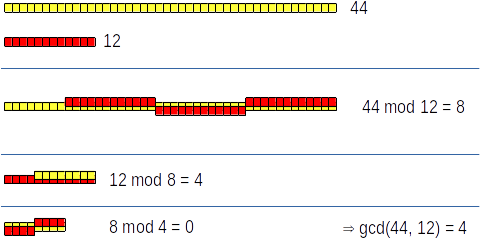
\includegraphics[width=\linewidth]{./gfx/Euclid-GCD}
\end{columns}
%
\end{frame}

% =========================================================================== %

\begin{frame}{Euclid's Algorithm: Analysis}
%
\begin{columns}
\column{.45\linewidth}
\begin{itemize}
\item Repeat steps \Thus Loop
	\begin{itemize}
	\item Find remainder
	\item Check if remainder is zero
	\item Update operands
	\end{itemize}
\item Termination condition
	\begin{itemize}
	\item Remainder is zero
	\item Unknown number of iterations (not \inPy{for ... range})
	\item No container to exhaust (not \inPy{for})
	\item[\Thus] \inPy{while}
	\item Result is smaller operand
	\end{itemize}
\end{itemize}
%
\column{.5\linewidth}
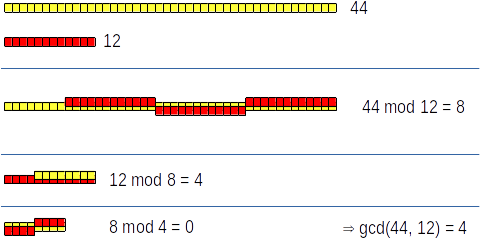
\includegraphics[width=\linewidth]{./gfx/Euclid-GCD}
\end{columns}
%
\begin{itemize}
\item Ordering Problem
	\begin{itemize}
	\item Implicitly required: $a \geq b$
	\item In fact not necessary due to property of modulus
	\end{itemize}
\end{itemize}
%
\end{frame}

% =========================================================================== %

\begin{frame}[fragile]
%
\begin{columns}
\column{.45\linewidth}
\begin{codebox}[GCD: Euclid's Algorithm]
\begin{minted}[linenos, fontsize=\scriptsize]{python3}
while b != 0:
    temp = b
    b = a % b
    a = temp

gcd = a
\end{minted}
\end{codebox}
%
\column{.48\linewidth}
\begin{itemize}
\item Updating operands requires temp copy
	\begin{itemize}
	\item Parallel update of \texttt{a} and \texttt{b}
	\item Evades ordering Problem
	\item Nifty Python Trick: hidden temp variable:
		\mint{python3}{a, b = b, a % b}
	\end{itemize}
\end{itemize}
\end{columns}
%
\begin{hintbox}[Length and Complexity]
Isn't it amazing how much thought can go into a mere five lines of code?

In this lies the \emph{art of coding}: Thinking through all possibilities and dealing with them without too much fuss
\end{hintbox}
%
\end{frame}

% =========================================================================== %

\begin{frame}{Algorithmic Elegance: Why Euclid Beats Brute Force}
%
\begin{itemize}
\item Concept: Runtime
	\begin{itemize}
	\item Number of steps to complete a task
	\item Complete mathematical theory
	\item[\thus] Numerics (each winter term)
	\item[\thus] Numerical Recipies (each winter term)
	\item[\thus] Algorithms and Data Structures (each summer term)
	\end{itemize}
\item Brute Force Approach
	\begin{itemize}
	\item Always takes $\min(a, b)$ steps
	\end{itemize}
\item Euclid
	\begin{itemize}
	\item Best case: takes 1 step
	\item Worst case: [difficult to compute; Wikipedia: $\propto \log(ab)$]
	\item Almost all cases: less steps than $\min(a, b)$
	\end{itemize}
\end{itemize}
%
\end{frame}
\end{document}

% MAREI!!
% whom do I give credit? Where?